%%%%%%%%%%%%%%%%%%%%%%%%%%%%%%%%%%%%%%%%%%%%%%%%%%%%
%%%%%%%%%%%%%%%%%%%%%% METHODS %%%%%%%%%%%%%%%%%%%%%
%%%%%%%%%%%%%%%%%%%%%%%%%%%%%%%%%%%%%%%%%%%%%%%%%%%%


% First, we will collect largest single-step potentiation gain seen in the lineage. 
% To our surprise, the initial work in Chapter \ref{chap:alife_submission} saw single mutations with substantial potentiation gain (at least 30 percentage points) in all four of the examined lineages. 
% This defied our initial expectation that single mutations can matter, but much of the potentiation is slowly accumulated over time. 
% Here, we will collect highest potentiation gain conferred from a single step to see if this trend holds beyond the four initial replicates. 
% Based on all four lineages having such potentiating mutations in Chapter \ref{chap:alife_submission}, I expect most lineages to have these potentiating mutations. 
% However, I also expect some portion of the lineages to not have any, but for them to slowly accumulate their potentiation. 
% This could occur if they traverse genotype space in such a way that multiple paths exist to reach learning, they do not depend on one particular mutation to start down the right path. 

% Looking in the opposite direction, we will also collect the largest potentiation \textit{loss} conferred by a single step in the lineage. 
% While we saw some evidence of decreasing potentiation in Chapter \ref{chap:alife_submission}, we did not detect single steps in the lineage that were particularly ``anti-potentiating''.
% My expectation is for mutations this strong to be present but rare. 
% These anti-potentiating mutations would likely be strongly beneficial mutations that move the lineage away from learning (e.g., toward an error-correcting reactive behavior). 
% One concern is that, in targeting the windows of large increases in potentiation, we are less likely to detect these anti-potentiating mutations. 
% This is why we will replay the additional ten lineages that do not evolve learning, switching our potentiation windows from the region that experiences the most potentiation gain to that which experiences the most potentiation loss. 
% The analyses of the non-learning lineage will otherwise be the same as those that evolved learning, but this will explore some possibilities of anti-potentiating mutations, if they exist in this system. 
% %However, if we find any evidence of them, future work could then do the opposite -- targeting decreases in potentiation -- to increase the likelihood of detecting them. 
% %Additionally, it is possible that this anti-potentiating mutations exist, but not in lineages that eventually evolve learning. 
% %Future work should look at the potentiation of learning in lineages that \textit{did not} evolve learning so see if single mutations led away from learning. 

% Before Chapter \ref{chap:alife_submission}, I expected most potentiating mutations to be either neutral or deleterious, because their lack of fitness benefit (or indeed, their fitness disadvantage) could factor in to their rarity and long-term potentiation effects. 
% However, of the four main potentiating mutations we found that two were neutral, one was deleterious, and one was beneficial. 
% Four mutations are clearly not enough to define a trend, so here we will again collect each mutations fitness effect compared to its parent. 
% While Chapter \ref{chap:alife_submission} did see a single beneficial potentiating mutation, I still expect most potentiating mutations to be neutral or deleterious.
% On the opposite side, I expect any anti-potentiating mutations we find to be strictly beneficial, though it is possible that they are merely potentiating future beneficial mutations that drag the lineage away from learning. 

% Finally, it is important to consider the context of the potentiating mutations. 
% As part of our analyses, we will check to see what behavior was performed by the lineage before and after the potentiating mutation. 
% I expect to see differences in the overall characteristics (potentiation change, phylogenetic distance to learning, etc.) between potentiation of lineages that evolved from reactive error correction to learning as compared to those that evolved straight from bet-hedged learning. 
% Similarly, I plan to analyze the number of steps in the lineage between the potentiating mutation and the first appearance of learning. 
% We saw considerable variation in this distance in Chapter \ref{chap:alife_submission}, and here I expect to see the same. 
% Additionally, we will ensure we look at both true distance in the lineage and \textit{meaningful} distance, as mutations to un-executed portions of the genome are just due to drift. 

% Look at epistatic interactions
% We could look at the performance of the first learning organism, and knockout the potentiating mutations. 
% My guess is that this should break learning in effectively every case

% Stats???

% \subsection{Analyses}

% Chapter \ref{02_alife_submission} explored the potentiation of four lineages capable of associative learning. 
% Here, I propose to greatly expand that scope by analyzing 50 different lineages. 
% First, this requires many more initial replicates in order to collect a suitable number of associative learning replicates to analyze. 

% The flow of exploratory replays followed by targeted replays in windows of potentiation increase will not change. 
% The analyses in Chapter \ref{02_alife_submission} focused on identifying the exact changes that potentiating mutations had on the genetic architecture of the organisms and how that interacted with later mutations to produce learning. 
% Here I propose to take a step back. 
% Investigating every potentiating mutation in all the lineages is infeasible in the time available to complete this dissertation. 
% Instead, I propose to extract specific statistics from each lineage to allow for meaningful comparisons to be made across lineages. 
% Of course, we do have the option to manually analyze individual mutations, but the core of this work will focus on this summary data. 

% First, we will collect information on potentiation changes much like we did in Chapter \ref{02_alife_submission}. 
% For each replayed lineage, we will collect the largest single-step potentiation increase and decrease, which will allow us to look into Hypotheses 1 and 2. 
% By analyzing the lineage data, we can also classify these potentiating and anti-potentiating mutations by their relative fitness effects, allowing us to test Hypotheses 3 and 4. 

% As demonstrated in Chapter \ref{02_alife_submission}, we classify each step in the lineage according to its behavior. 
% This will allow us to compare potentiating mutations based on what behavioral background they occurred on. 
% Therefore, we can compare across behaviors to test Hypothesis 5. 

% Finally, we can identify the potentiating step in the lineage and the step where learning first appears. 
% By analyzing the steps between these two points, we can begin to investigate Hypothesis 6. 
% However, we will also need to differentiate between all mutations and ``meaningful'' mutations.
% While working on Chapter \ref{02_alife_submission}, we noticed that many organisms had regions of their genotype that were not executed before or after learning. 
% Thus it is important that we exclude mutations to these regions, as they have no effect on the organism's behavior. 

\section{Hypotheses}

\begin{enumerate}
    \item Successful lineages often see substantial increases in potentiation conferred by a single mutation
    \item Many successful lineages encounter substantial losses in potentiation
    \item Most potentiating mutations are either neutral or deleterious when they occur
    \item Most ``anti-potentiating'' mutations are beneficial when they occur
    \item The type of pre-learning behavior exhibited by the lineage will influence the type of potentiation that occurs
    \item Most potentiating mutations occur long before learning actually appears in the lineage
\end{enumerate}





%%%% Results
% \begin{figure}[h!]
% \begin{center}
% 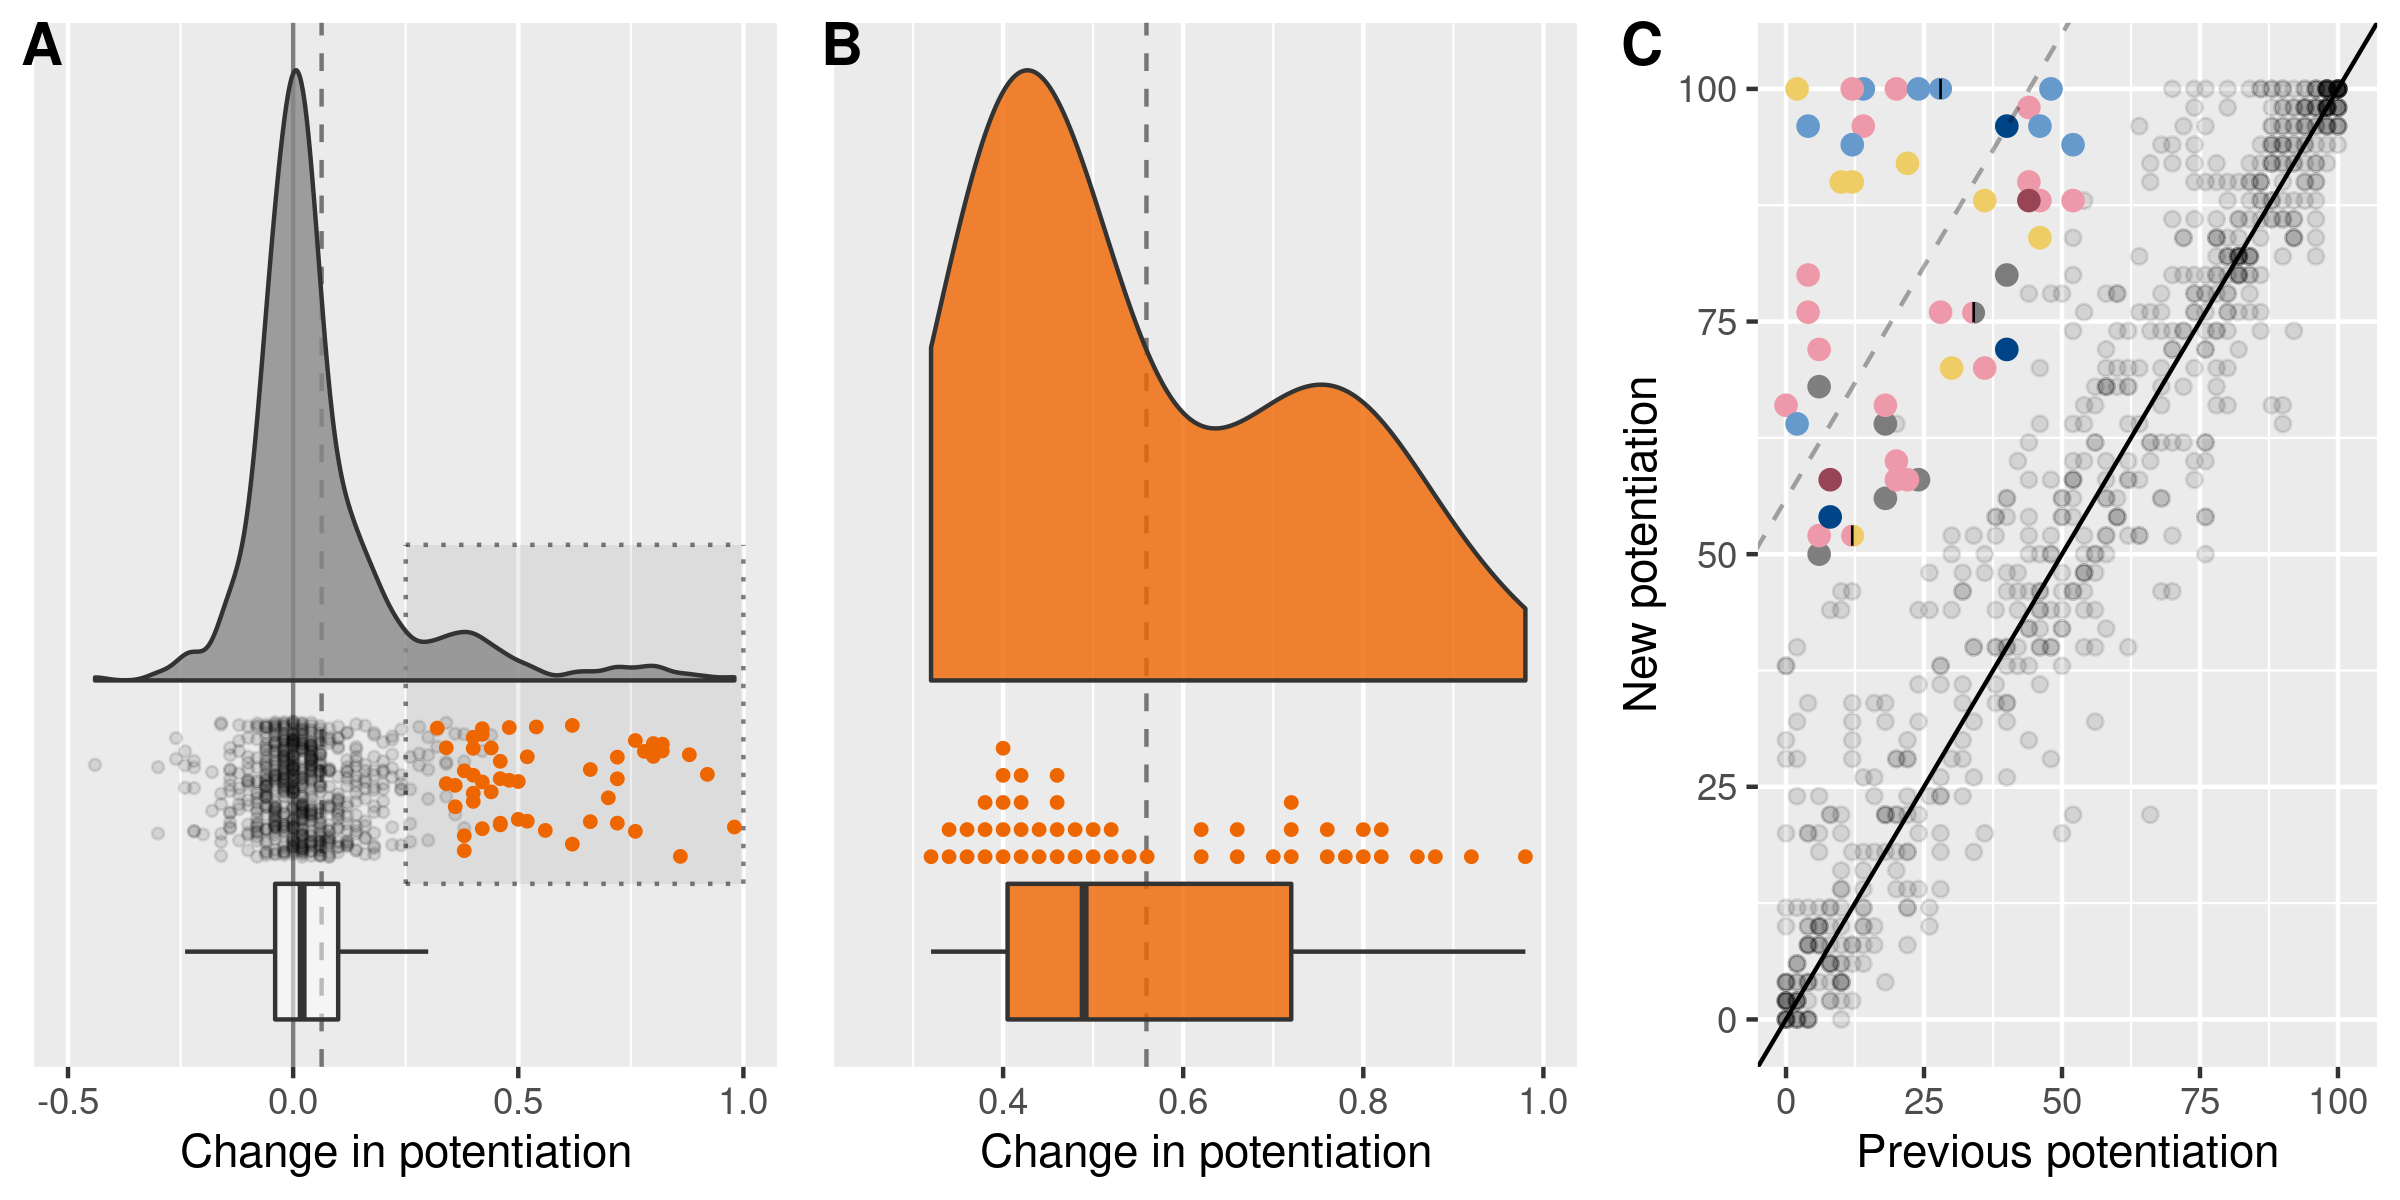
\includegraphics[width=0.9\textwidth]{03_replaying_associative_learning/media/exploratory_replays.png}
% \end{center}
% \caption{ 
% Aggregate data for the \textit{exploratory} replays of learning replicates. 
% \textbf{Subplot A)} Raincloud plot showing the distribution of potentiation changes for \textit{all} replayed windows.
% The solid vertical line shows zero change, the dashed vertical line shows the mean of the potentiation changes, and the shaded region shows the area displayed by Subplot B. 
% \textbf{Subplot B)}  Raincloud plot showing the distribution of maximum single-window potentation change for each replicate (one point for each of the 50 learning replicates). 
% The dashed vertical line shows the mean of these changes. 
% \textbf{Subplot C)} A scatter plot showing the potentiation before and after each exploratory window. 
% The largest potentiation gain per replicate is shown in color corresponding to the behavioral phenotype at the end of the window (see Figure \ref{fig:initial_reps} for color key). 
% Split circles show two replicates at the same point. 
% Semi-transparent points show the rest of the per-window potentiation changes. 
% The line shows $y=x$. 
% Potentiation gain is thus the vertical distance to this line. 
% The dashed line shows is the same as Subplot B. 
% }\label{fig:exploratory_replays}
% \end{figure}



% \begin{figure}[h!]
% \begin{center}
% 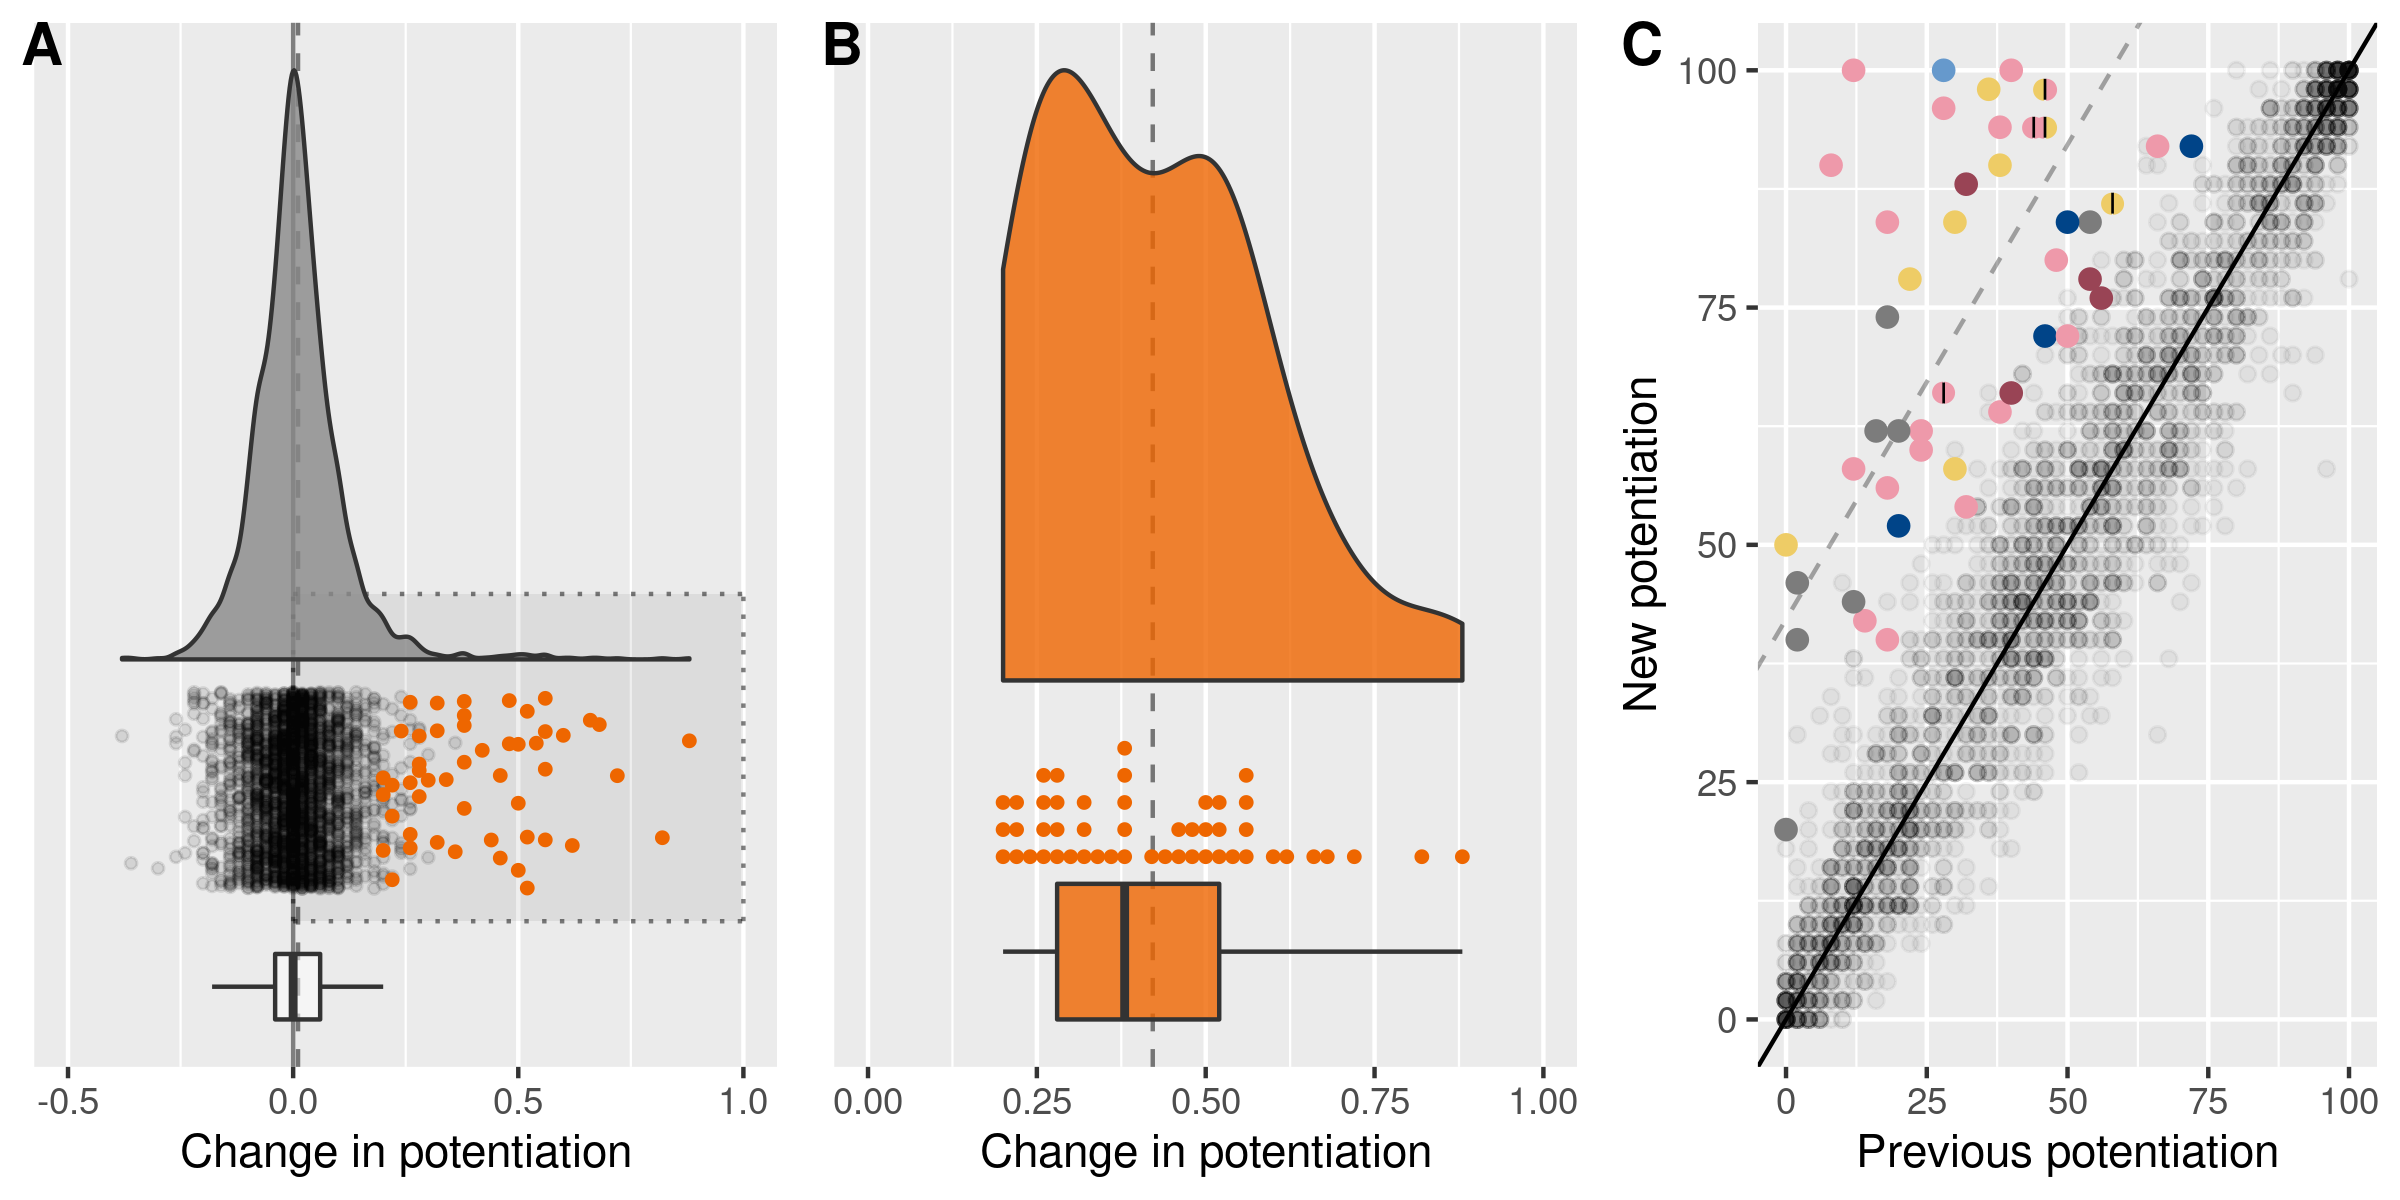
\includegraphics[width=0.9\textwidth]{03_replaying_associative_learning/media/targeted_replays.png}
% \end{center}
% \caption{ 
% Aggregate data for the \textit{targeted} replays of learning replicates. 
% \textbf{Subplot A)} Raincloud plot showing the distribution of potentiation changes for \textit{all} replayed lineage steps.
% The solid vertical line shows zero change, the dashed vertical line shows the mean of the potentiation changes, and the shaded region shows the area displayed by Subplot B. 
% \textbf{Subplot B)}  Raincloud plot showing the distribution of maximum single-step potentation change for each replicate. 
% The dashed vertical line shows the mean of these changes. 
% \textbf{Subplot C)} A scatter plot showing the potentiation before and after each replayed lineage step. 
% The largest per-step potentiation gain per replicate is shown in color corresponding to the behavioral phenotype at the end of the window (see Figure \ref{fig:initial_reps} for color key). 
% Split circles show two replicates at the same point. 
% Semi-transparent points show the rest of the per-window potentiation changes. 
% The line shows $y=x$, and potentiation gain is thus the vertical distance to this line. 
% The dashed line shows is the same as Subplot B. 
% }\label{fig:targeted_replays}
% \end{figure}

% Show histogram of maximum potentiation jump per replicate
% Show histogram of all potentiation changes?
% Show instances of large and small jumps?

% \begin{figure}[ht!]
% \begin{center}
% 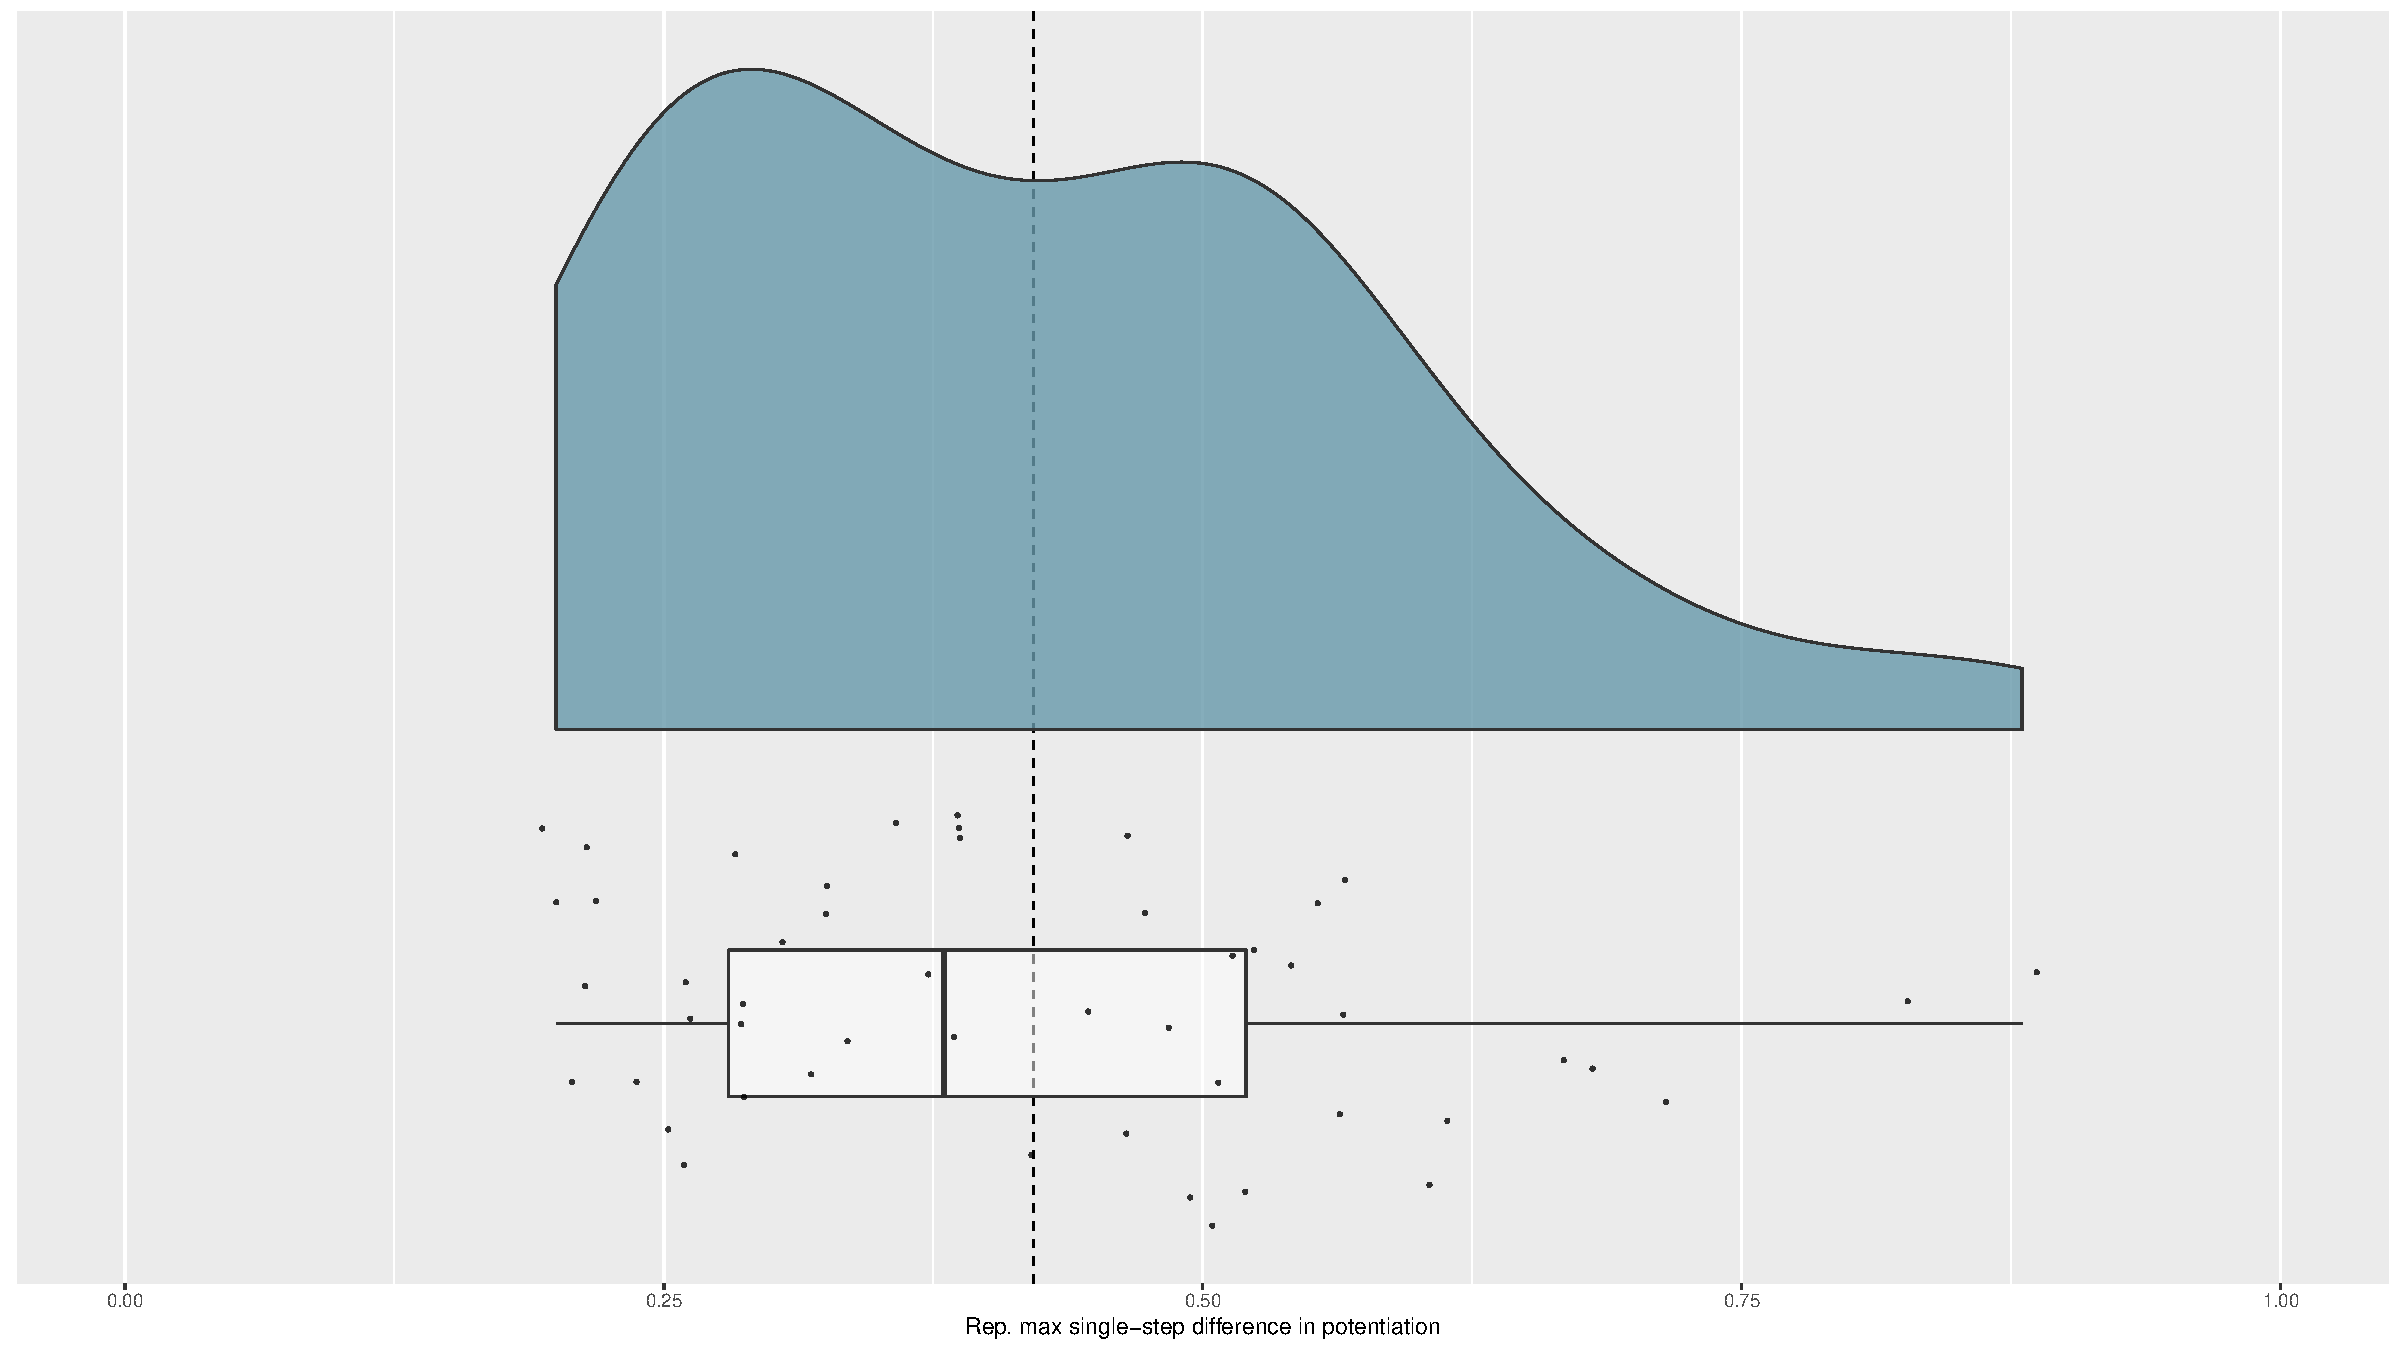
\includegraphics[width=0.9\textwidth]{03_replaying_associative_learning/media/potentiation/largest_potentiation_differences_large_raincloud.pdf}
% \end{center}
% \caption{ 
% A raincloud plot of the largest gain in potentiation conferred with a single phylogenetic step for each of the 50 analyzed learning lineages. 
% The dashed line shows the mean of the data.
% }\label{fig:potentiation:largest_jump_raincloud}
% \end{figure}



% \subsection{Potentiating mutations are not limited by fitness effect}
% % Show bar chart of how many replicates experienced each fitness effect
% % Show optimality somehow?

% \begin{figure}[h!]
% \begin{center}
% 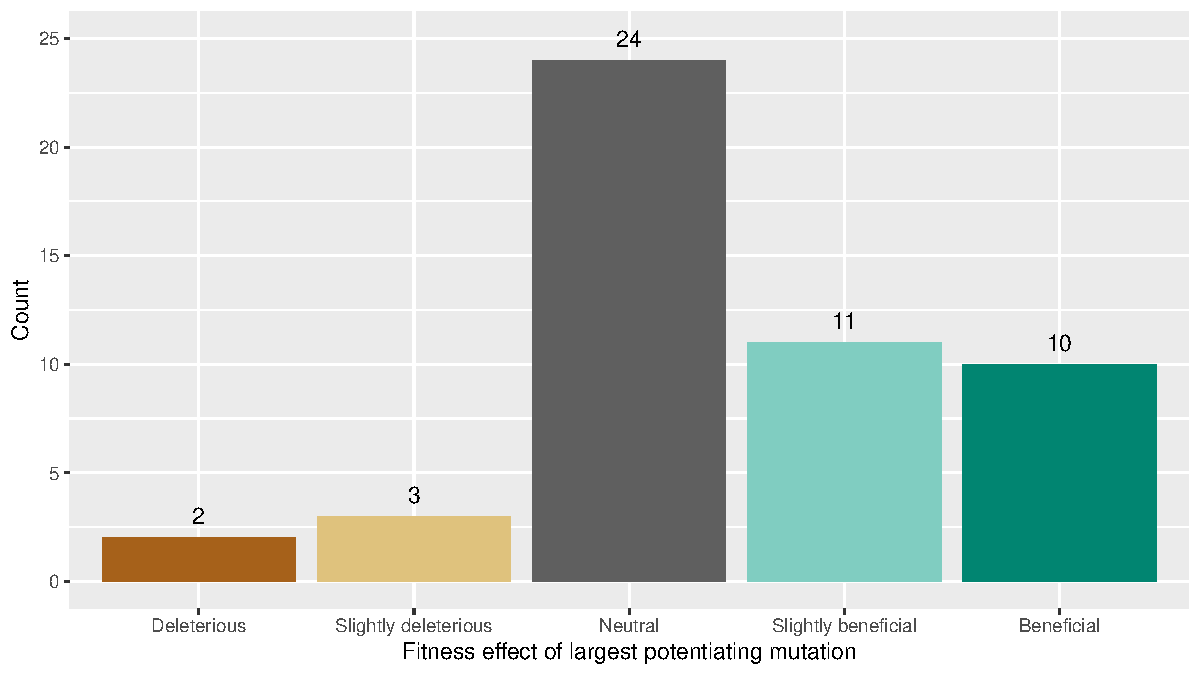
\includegraphics[width=0.9\textwidth]{03_replaying_associative_learning/media/fitness_effects/fitness_effect_classification_largest_step_counts_small.pdf}
% \end{center}
% \caption{ 
% Each of the 50 learning replicates that we replayed had one phylogenetic step that conferred the largest gain in potentiation. 
% These bars show how many of those 50 steps fell into each fitness classification.  
% }\label{fig:fitness_effect:counts}
% \end{figure}

Figure \ref{fig:fitness_effect:counts} categorizes the fitness effect for phylogenetic step that saw the largest increase in potentiation for each of the 50 learning replicates we analyzed. 
Deleterious, neutral, and beneficial steps are all represented. 
However, 90\% of these potentiating steps had a neutral or better effect on fitness. 

% \begin{figure}[h!]
% \begin{center}
% 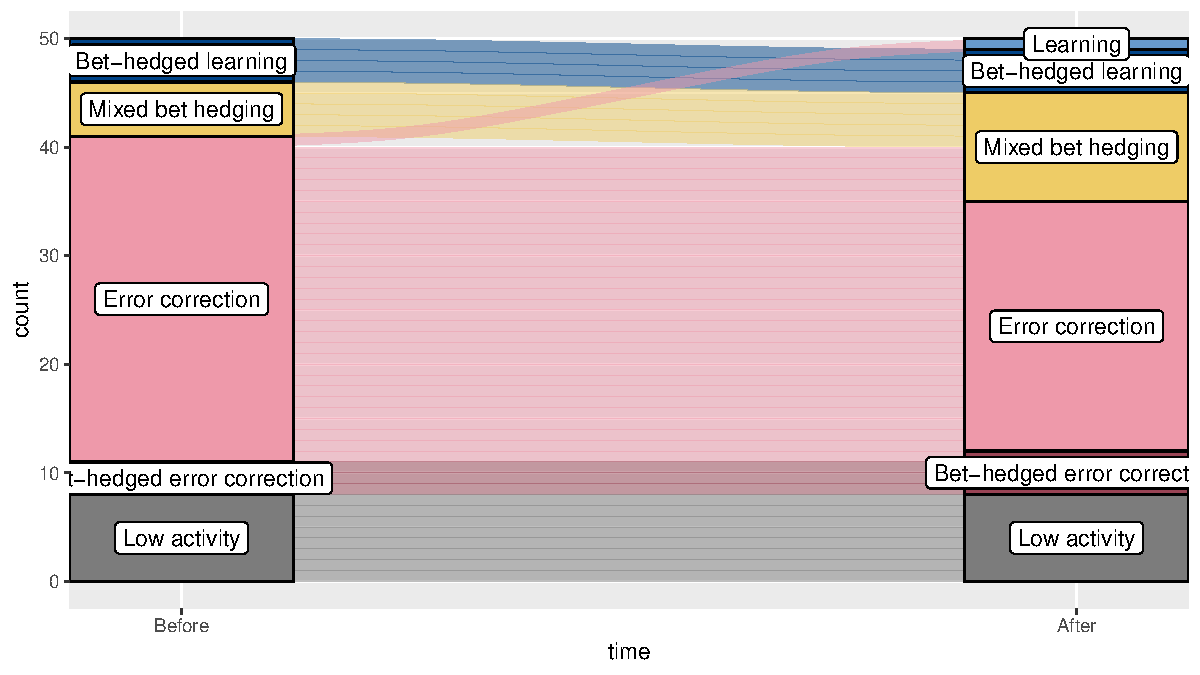
\includegraphics[width=0.9\textwidth]{figures/behavior_classification/behavior_alluvial_2.pdf}
% \end{center}
% \caption{ 
% Each of the 50 learning replicates that we replayed had one mutational step that conferred the largest gain in potentiation. 
% These bars show how many of those 50 steps fell into each fitness classification.  
% }\label{fig:fitness_effect:counts}
% \end{figure}

% \begin{center}
%     \begin{tabular}{|c|c|}
%         \hline
%         \thead{Condition} & \thead{Count} \\
%         \hline
%          Single mutation & 30 \\
%          Two mutations & 14 \\
%          Three mutations & 3 \\
%          Four mutations & 1 \\
%          Five mutations & 2 \\
%          \hline
%     \end{tabular}
% \end{center}
